\documentclass[10pt, aspectratio=169]{slidesiffmodelo}
\usepackage{amsmath,amssymb}
\usepackage{booktabs}
\usepackage{xcolor}
\usepackage{graphicx}
\usepackage{tikz}
\usetikzlibrary{shapes,arrows,positioning}
% Configuração de Modelo Branco (Claro) — Paleta Institucional
\definecolor{iffred}{RGB}{185, 28, 28}
\definecolor{iffgreen}{RGB}{21, 128, 61}
\definecolor{iffblue}{RGB}{37, 99, 235}
\definecolor{iffgold}{RGB}{180, 83, 9}
\definecolor{ifforange}{RGB}{194, 65, 12}
\definecolor{iffviolet}{RGB}{109, 40, 217}
\definecolor{ifflight}{RGB}{248, 250, 252}
\setbeamercolor{normal text}{fg=black!90,bg=white}
\setbeamercolor{structure}{fg=iffgreen}
\setbeamercolor{title}{fg=iffred}
\setbeamercolor{frametitle}{fg=iffred}
\setbeamercolor{item}{fg=iffgreen}
\setbeamercolor{subitem}{fg=iffgold}
% Estrutura de Cabeçalho e Rodapé IDÊNTICA ao PPTX Institucional
\setbeamertemplate{headline}{%
  \vspace{0.18cm}%
  \hspace{0.5cm}%
  \begin{minipage}{0.35\linewidth}%
    \includegraphics[height=0.65cm]{img/logoiff.png}%
  \end{minipage}%
  \hfill%
  \begin{minipage}{0.55\linewidth}%
    \raggedleft\footnotesize\textbf{\color{iffred} LaTeX e Escrita Acadêmica --- NBR 14724}%
  \end{minipage}%
  \hspace{0.5cm}%
  \vspace{0.12cm}%
  {\color{iffgold}\hrule height 1.2pt}%
}
\setbeamertemplate{footline}{%
  {\color{iffgold}\hrule height 0.8pt}%
  \vspace{0.1cm}%
  \hspace{0.5cm}%
  \begin{minipage}{0.35\linewidth}%
    \scriptsize\textbf{\color{iffgreen} Pedro Henrique Rocha de Andrade}%
  \end{minipage}%
  \hfill%
  \begin{minipage}{0.35\linewidth}%
    \centering\scriptsize\textbf{\color{ifforange} IFF Bom Jesus do Itabapoana}%
  \end{minipage}%
  \hfill%
  \begin{minipage}{0.15\linewidth}%
    \raggedleft\scriptsize\textbf{\color{iffviolet} \insertframenumber{} / \inserttotalframenumber}%
  \end{minipage}%
  \hspace{0.5cm}%
  \vspace{0.15cm}%
}
\title{Aula 09: Aula 9 \\ \small Sub}
\author{\textbf{Pedro Henrique Rocha de Andrade}\inst{1}}
\institute{\inst{1} Instituto Federal Fluminense --- \textit{Campus} Bom Jesus do Itabapoana}
\date{\today}
\begin{document}
\begin{frame}[t]
    \titlepage
    \begin{tikzpicture}[remember picture, overlay]
      \node[anchor=east, xshift=-1cm, yshift=1.5cm] at (current page.east) {\includegraphics[width=2.5cm]{img/qrcode_transparente.png}};
    \end{tikzpicture}
\end{frame}

\begin{frame}[t]
    \frametitle{Sumário da Aula}
    \tableofcontents
\end{frame}

\section{Desenvolvimento Teórico e Metodológico}
\begin{frame}[t]
    \frametitle{\color{iffgold}1. O Capítulo de Resultados}
    \begin{itemize}
        \item \textcolor{iffgreen}{\textbf{[Importante]} O capítulo de ''Resultados'' (frequentemente agrupado como ''Resultados e Discussão'', embora a divisão seja a preferida em pesquisas experimentais exatas) é o destino final e razão de existir de toda a argumentação da pesquisa.}
        \item \textcolor{iffviolet}{\textbf{[Para a Prova]} Para que os resultados possuam clareza e credibilidade, os dados devem ser apresentados em um formato visual estruturado e padronizado. Na escrita acadêmica brasileira (e exigido pelo \texttt{ifftese} no LaTeX), há uma forte distinção formal entre a exibição de dados estatísticos/numéricos e a exibição de conteúdos qualitativos e textuais. Esta separação é baseada conjuntamente na NBR 14724 da ABNT e nas normas de apresentação tabular do IBGE.}
    \end{itemize}
\end{frame}

\begin{frame}[t]
    \frametitle{\color{iffgold}2. A Confusão Histórica: Tabelas vs. Quadros}
    \begin{itemize}
        \item \textcolor{iffgreen}{\textbf{[Importante]} Muitos alunos iniciantes cometem um erro crasso e frequente nas dissertações: chamam qualquer arranjo de linhas e colunas de ''Tabela''. Para a norma técnica no Brasil, existem duas classes fundamentais e distintas, com formatações visuais rigorosamente diferentes: as Tabelas (Norma IBGE) e os Quadros (ABNT).}
        \item \textcolor{iffblue}{\textbf{[Vale Lembrar]} 2.1 Tabela (Segundo as Normas de Apresentação Tabular do IBGE, 1993)}
        \item \textbf{Propósito:} Exibir dados numéricos, estatísticos e matemáticos sujeitos a análise quantitativa. O foco absoluto da tabela é evidenciar as variáveis métricas em suas colunas, facilitando a leitura de séries numéricas contínuas e permitindo comparações rápidas de ordens de grandeza.
        \item \textcolor{iffgreen}{\textbf{[Importante]} \textbf{Regras de Formatação Estritas (IBGE 1993):}}
    \end{itemize}
\end{frame}

\begin{frame}[t]
    \frametitle{\color{iffgold}2. A Confusão Histórica: Tabelas vs. Quadros (Cont.)}
    \begin{itemize}
        \item \textcolor{iffgreen}{\textbf{[Importante]} 1.  \textbf{Sem Bordas Laterais:} A característica visual mais marcante da Tabela do IBGE é que ela \textbf{não possui traços verticais delimitando suas bordas direita e esquerda externas}.}
        \item \textcolor{iffviolet}{\textbf{[Para a Prova]} 2.  \textbf{Sem Grades Internas Completas:} Evita-se fechar células como num tabuleiro da velha. Há traços horizontais demarcando o cabeçalho superior e traços horizontais finalizando a parte inferior da tabela. Traços verticais internos são desencorajados, usados apenas em tabelas imensamente complexas (mas ainda sem borda externa).}
        \item 3.  \textbf{Posição do Título:} O título localiza-se na parte superior, antecedido da palavra Tabela e de seu número de ordem em arábicos (ex: Tabela 1 - Desempenho do Algoritmo Genético).
        \item \textcolor{iffgreen}{\textbf{[Importante]} 4.  \textbf{Fonte da Informação:} É obrigatório citar a fonte dos dados no rodapé da tabela, mesmo que a fonte seja o próprio autor da pesquisa (ex: Fonte: Elaborado pelo autor (2026)). A fonte deve vir na parte inferior.}
    \end{itemize}
\end{frame}

\begin{frame}[t]
    \frametitle{\color{iffgold}2. A Confusão Histórica: Tabelas vs. Quadros (Cont.)}
    \begin{itemize}
        \item \textcolor{iffgreen}{\textbf{[Importante]} 5.  \textbf{Corpo e Cabeçalho:} O cabeçalho deve ser simples, explicando as variáveis (ex: Tempo (ms), Tensão (V), Erro (\%)).}
        \item \textcolor{iffblue}{\textbf{[Vale Lembrar]} 2.2 Quadro (ABNT NBR 14724)}
        \item \textbf{Propósito:} Exibir e sintetizar dados predominantemente qualitativos, textuais, conceitos, classificações, equações alfanuméricas, organogramas comparativos ou strings lógicas de revisão sistemática.
        \item \textcolor{iffgreen}{\textbf{[Importante]} \textbf{Regras de Formatação Estritas (ABNT):}}
    \end{itemize}
\end{frame}

\begin{frame}[t]
    \frametitle{\color{iffgold}2. A Confusão Histórica: Tabelas vs. Quadros (Cont.)}
    \begin{itemize}
        \item \textcolor{iffgreen}{\textbf{[Importante]} 1.  \textbf{Bordas Completamente Fechadas:} O Quadro é uma ''caixa'' perfeitamente fechada. Todas as suas bordas externas e as grandes internas (verticais e horizontais) devem estar desenhadas, delimitando perfeitamente as células de texto.}
        \item \textcolor{iffviolet}{\textbf{[Para a Prova]} 2.  \textbf{Identificação:} Assim como a tabela, possui título na parte superior e numeração sequencial (ex: Quadro 1 - Critérios de Inclusão da Revisão Bibliográfica).}
        \item 3.  \textbf{Fonte da Informação:} A fonte deve ser citada no rodapé da figura (ex: Fonte: Adaptado de Silva (2022)).
    \end{itemize}
\end{frame}

\begin{frame}[t]
    \frametitle{\color{iffgold}3. Implementação Prática no LaTeX}
    \begin{itemize}
        \item \textcolor{iffgreen}{\textbf{[Importante]} A classe \texttt{ifftese} e pacotes como o \texttt{booktabs} (para tabelas de alta qualidade) tratam dessas diferenças estruturais de forma nativa e profissional.}
        \item \textcolor{iffviolet}{\textbf{[Para a Prova]}   Para criar \textbf{Tabelas} visualmente belas, sem bordas laterais e com espaçamento elegante, utiliza-se quase sempre o pacote \texttt{booktabs} com os comandos \texttt{\toprule}, \texttt{\midrule} e \texttt{\bottomrule}, evitando os traços verticais \texttt{|} no ambiente \texttt{tabular}.}
        \item   Para criar \textbf{Quadros}, o LaTeX precisa fechar todas as grades. Geralmente usa-se a própria estrutura nativa do \texttt{tabular} (ex: \texttt{\begin{tabular}{|c|c|c|}}) junto com um ambiente flutuante específico como \texttt{\begin{quadro}} (criado no preâmbulo por meio de pacotes de customização ou pela classe da universidade).
    \end{itemize}
\end{frame}

\begin{frame}[t]
    \frametitle{\color{iffgold}4. Diagrama Comparativo (Mermaid)}
    \begin{itemize}
        \item \textcolor{iffgreen}{\textbf{[Importante]} D[Dado a Apresentar] --> E{Numérico/Estatístico?};}
        \item \textcolor{iffviolet}{\textbf{[Para a Prova]} E -- Sim (Valores métricos) --> T[Usar TABELA - Norma IBGE];}
        \item E -- Não (Textos, Conceitos) --> Q[Usar QUADRO - Norma ABNT];
        \item \textcolor{iffgreen}{\textbf{[Importante]} T --> T1[Laterais ABERTAS \n Sem traços verticais nas bordas];}
    \end{itemize}
\end{frame}

\begin{frame}[t]
    \frametitle{\color{iffgold}4. Diagrama Comparativo (Mermaid) (Cont.)}
    \begin{itemize}
        \item \textcolor{iffgreen}{\textbf{[Importante]} T --> T2[Bordas superior e inferior fechadas \n com fios grossos/finos];}
        \item \textcolor{iffviolet}{\textbf{[Para a Prova]} Q --> Q1[Laterais FECHADAS \n Grade completa como gradeado];}
        \item Q --> Q2[Todas as células delimitadas];
        \item \textcolor{iffgreen}{\textbf{[Importante]} style T fill:\#ffccbc,stroke:\#d84315}
    \end{itemize}
\end{frame}

\begin{frame}[t]
    \frametitle{\color{iffgold}4. Diagrama Comparativo (Mermaid) (Cont.)}
    \begin{itemize}
        \item \textcolor{iffgreen}{\textbf{[Importante]} style Q fill:\#c5cae9,stroke:\#283593}
    \end{itemize}
\end{frame}

\begin{frame}[t]
    \frametitle{\color{iffgold}5. Estudo de Caso}
    \begin{itemize}
        \item \textcolor{iffgreen}{\textbf{[Importante]} \textbf{O Cenário:} O mestrando João avaliou 3 linguagens de programação diferentes (C, Python e Java) para criptografia embarcada num chip IoT. Ele quer mostrar as vantagens teóricas de cada uma, e também mostrar os resultados medidos de uso de CPU e tempo gasto para criptografar.}
        \item \textcolor{iffviolet}{\textbf{[Para a Prova]} \textbf{Solução Híbrida e Correta:}}
        \item 1.  Para exibir os parâmetros conceituais e características operacionais de cada linguagem, João cria o \textbf{Quadro 1 - Comparativo qualitativo das linguagens estudadas}. O quadro terá linhas verticais e horizontais fechadas. Nas colunas: ''Linguagem'', ''Tipagem'', ''Paradigma'', ''Vantagem no IoT''. O conteúdo das células será textual (ex: ''Fortemente tipada'', ''Orientação a objetos'').
        \item \textcolor{iffgreen}{\textbf{[Importante]} 2.  Para exibir os resultados finais experimentais recolhidos de seus sensores na bancada, ele cria a \textbf{Tabela 1 - Desempenho computacional dos algoritmos criptográficos em IoT}. A tabela não terá bordas laterais. As colunas serão: ''Linguagem'', ''Tempo de Execução (ms)'', ''Uso de CPU (\%)'', ''Consumo Estimado (mW)''. O interior será preenchido com números de ponto flutuante, médias e desvio-padrão obtidos do experimento.}
    \end{itemize}
\end{frame}

\begin{frame}[t]
    \frametitle{\color{iffgold}6. Exercício Prático}
    \begin{itemize}
        \item \textcolor{iffgreen}{\textbf{[Importante]} 1.  Considere os seguintes dados: O Brasil foi pentacampeão do mundo nos anos de 1958, 1962, 1970, 1994 e 2002. A Itália foi tetracampeã em 1934, 1938, 1982, 2006. A Alemanha tetracampeã em 1954, 1974, 1990, 2014. Você classificaria essa informação visualmente num Quadro ou numa Tabela? Por quê?}
        \item \textcolor{iffviolet}{\textbf{[Para a Prova]} 2.  No ambiente LaTeX \texttt{tabular}, como você declararia as colunas para uma \textbf{Tabela} (IBGE) de 3 colunas centralizadas, respeitando a ausência de bordas externas verticais?}
        \item 3.  E como faria a declaração do mesmo ambiente \texttt{tabular} para o \textbf{Quadro} (ABNT) com as mesmas 3 colunas centralizadas, de forma que houvesse traços verticais delimitando todas as colunas e bordas externas?
    \end{itemize}
\end{frame}

\section{Síntese Arquitetural do Ecossistema}
\begin{frame}[t]
    \frametitle{Hierarquia e Fluxo Documental na ABNT (Diagrama TikZ)}
    \begin{center}
    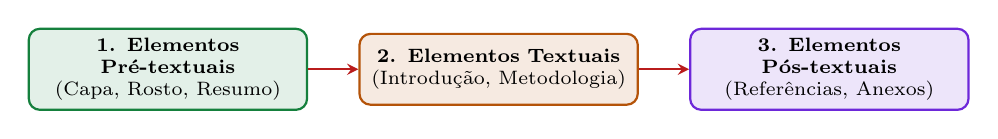
\begin{tikzpicture}[node distance=1.6cm, auto,
        boxpre/.style={rectangle, draw=iffgreen, thick, fill=iffgreen!12!white, text width=3.3cm, align=center, rounded corners, minimum height=0.9cm, font=\scriptsize},
        boxtex/.style={rectangle, draw=iffgold, thick, fill=iffgold!12!white, text width=3.3cm, align=center, rounded corners, minimum height=0.9cm, font=\scriptsize},
        boxpos/.style={rectangle, draw=iffviolet, thick, fill=iffviolet!12!white, text width=3.3cm, align=center, rounded corners, minimum height=0.9cm, font=\scriptsize},
        arrow/.style={->, >=stealth, thick, color=iffred}
    ]
        \node[boxpre] (pre) {\textbf{1. Elementos Pré-textuais}\\ (Capa, Rosto, Resumo)};
        \node[boxtex, right of=pre, xshift=2.6cm] (tex) {\textbf{2. Elementos Textuais}\\ (Introdução, Metodologia)};
        \node[boxpos, right of=tex, xshift=2.6cm] (pos) {\textbf{3. Elementos Pós-textuais}\\ (Referências, Anexos)};
        \draw[arrow] (pre) -- (tex);
        \draw[arrow] (tex) -- (pos);
    \end{tikzpicture}
    \end{center}
    \vspace{0.3cm}
    \begin{itemize}
        \item \textbf{Fluxo de Compilação:} Separação estrita entre conteúdo semântico (.tex) e regras tipográficas (.cls/.sty);
        \item \textbf{Automação:} Gerenciamento dinâmico de referências cruzadas, paginação e listas preliminares.
    \end{itemize}
\end{frame}

\section{Referências Bibliográficas}
\begin{frame}[t,allowframebreaks]
    \frametitle{Referências Bibliográficas}
    \begin{thebibliography}{99}
    \bibitem{nbr14724} ASSOCIAÇÃO BRASILEIRA DE NORMAS TÉCNICAS. \textit{NBR 14724: Informação e documentação --- Trabalhos acadêmicos --- Apresentação.} Rio de Janeiro: ABNT, 2011.
    \bibitem{nbr10520} ASSOCIAÇÃO BRASILEIRA DE NORMAS TÉCNICAS. \textit{NBR 10520: Informação e documentação --- Citações em documentos --- Apresentação.} Rio de Janeiro: ABNT, 2023.
    \bibitem{nbr6023} ASSOCIAÇÃO BRASILEIRA DE NORMAS TÉCNICAS. \textit{NBR 6023: Informação e documentação --- Referências --- Elaboração.} Rio de Janeiro: ABNT, 2018.
    \bibitem{ibge1993} INSTITUTO BRASILEIRO DE GEOGRAFIA E ESTATÍSTICA (IBGE). \textit{Normas de apresentação tabular.} 3. ed. Rio de Janeiro: IBGE, 1993.
    \bibitem{page2021} PAGE, M. J. et al. The PRISMA 2020 statement: an updated guideline for reporting systematic reviews. \textit{BMJ}, v. 372, n. 71, 2021.
    \end{thebibliography}
\end{frame}

\section{Fechamento}
\begin{frame}[t]
    \frametitle{Obrigado!}
    \begin{textoimagem}
        \textbf{Pedro Henrique Rocha de Andrade}\\
        Instituto Federal Fluminense (\textit{Campus} Bom Jesus do Itabapoana)\\
        \email\\
        \vspace{0.4cm}
        Dúvidas ou sugestões? Acesse o portal institucional da disciplina e faça o download dos pacotes apontando para o QR Code ao lado.
    \colunaimagem
        \inserirfigura[width=0.65\linewidth]{img/qrcode_transparente.png}{Acesso Institucional ao Curso}{}{fig:qrcode}
    \end{textoimagem}
\end{frame}

\end{document}